\section{Rechenarten}
	\begin{multicols}{2}
		\subsection{Einerkomplement}
			Das Einerkomplement wird durch Invertieren aller Bits der positiven Zahl gebildet.\\
			$\mathbf{A_{k1}=\overline{A}}$\\
			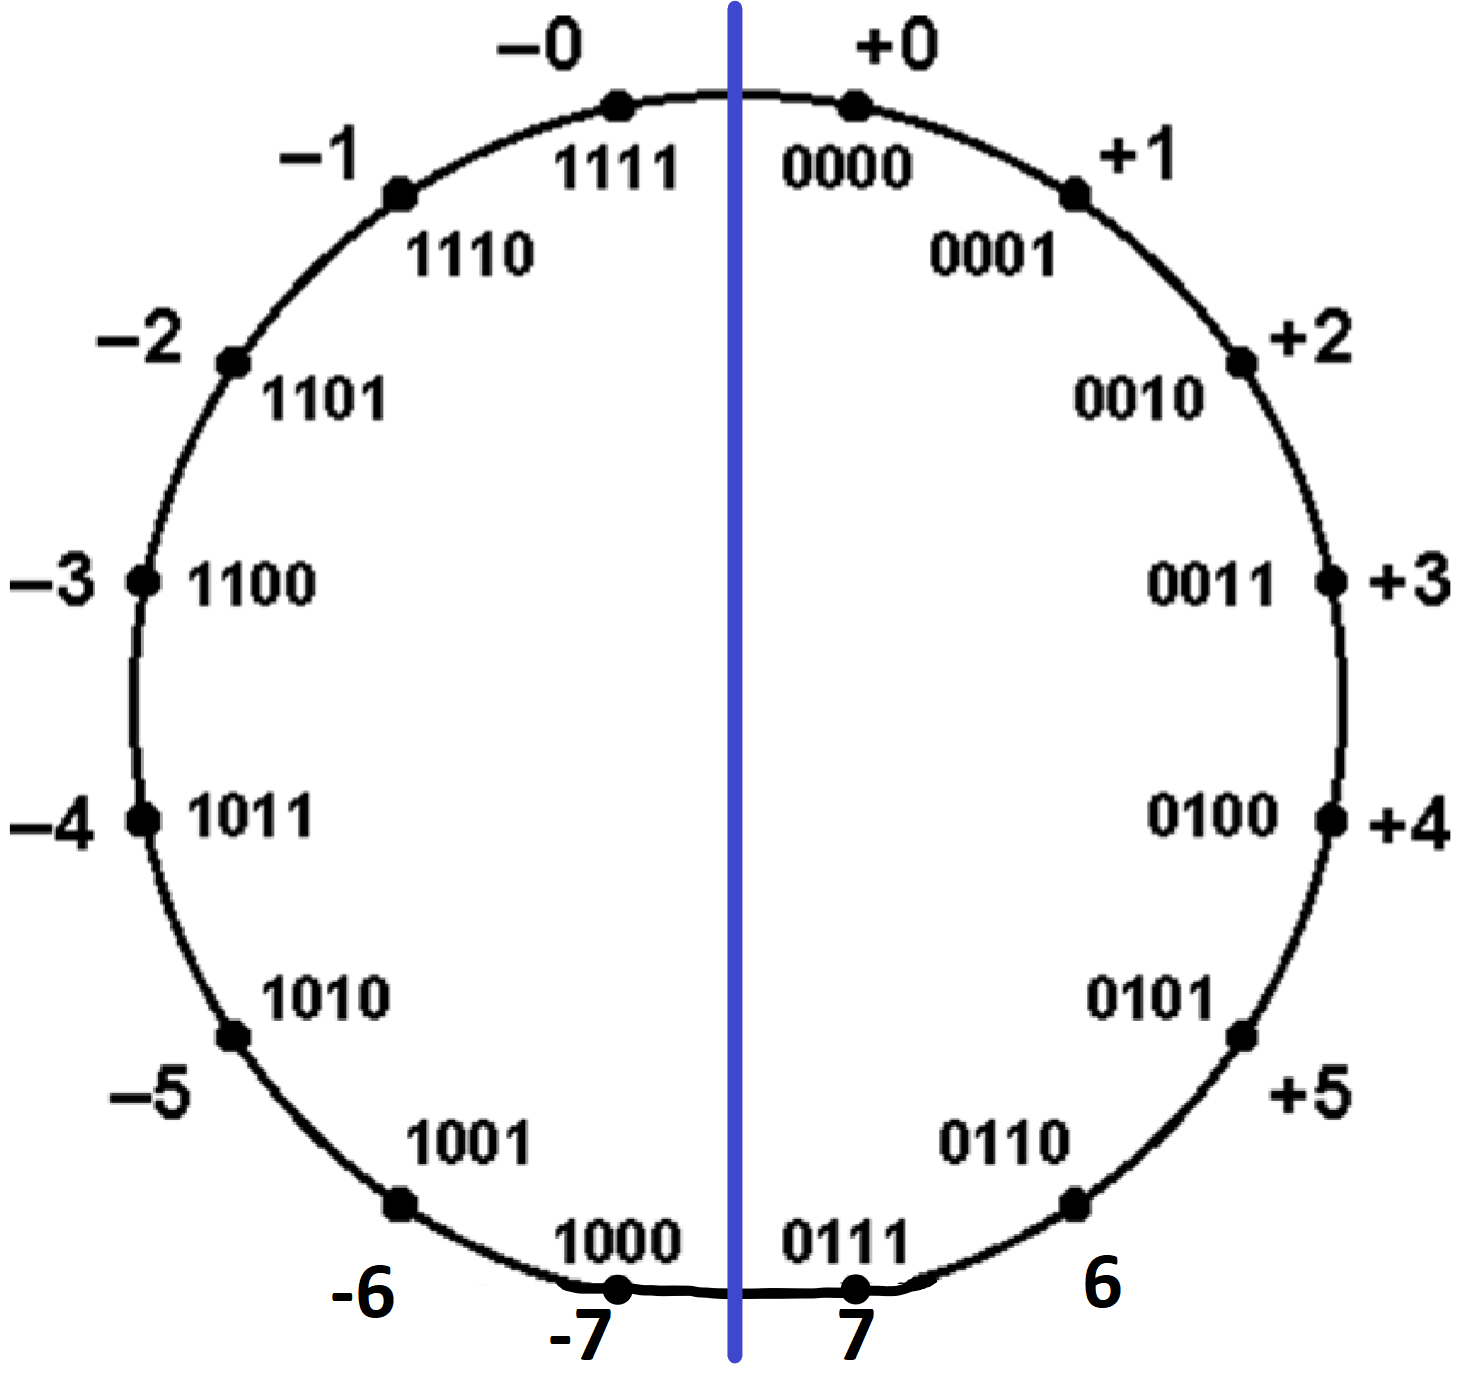
\includegraphics[width=0.4\textwidth]{pics/zahlensysteme/einerkomplement.png}	
			\columnbreak
			
		\subsection{Zweierkomplement}
			Das Zweierkomplement wird durch Invertieren aller Bits der positiven Zahl und der Addition von 1 gebildet.\\
			$\mathbf{A_{k2}=\overline{A}+1}=(2^n-A)$\\
			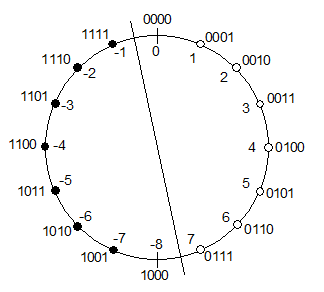
\includegraphics[width=0.4\textwidth]{pics/zahlensysteme/zweierkomplement.png}
	\end{multicols}

\subsection{Addition}
	\begin{multicols}{3}
		\subsubsection{Ganzzahlen}
		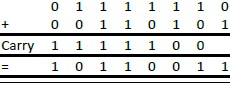
\includegraphics[width=0.3\textwidth]{pics/zahlensysteme/addition1.jpg}
		%\columnbreak
		
		\subsubsection{Festkommazahlen}
		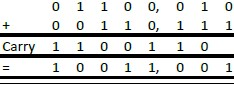
\includegraphics[width=0.3\textwidth]{pics/zahlensysteme/addition2.jpg}
		%\columnbreak
		
		\subsubsection{Vorzeichen-Darstellung}
		\begin{minipage}[c]{1.5 cm}
			Es gilt: 
			\newline
		\end{minipage}
		\begin{minipage}[c]{3.5 cm}
			\begin{compactitem}
				\item 0$\rightarrow$positiv
				\item 1$\rightarrow$negativ
			\end{compactitem}
		\end{minipage}
		Beispiel:\\
		\begin{tabular}{llll}
			$+$ & 12310 & = & 0 111 1011\\
			$-$ & 12310 & = & 1 111 1011\\
		\end{tabular}
	\end{multicols}

\subsection{Subtraktion}
	F"ur die Subtraktion A$-$B=C sind folgende Schritte notwendig:
	\begin{compactitem}
		\item 1) Der Subtrahend B muss ins Zweierkomplement gebracht werden.
		\item 2) Die arithmetische Operation muss durchgef"uhrt werden.
		\item 3) Das Resultat muss korrekt interpretiert werden.
	\end{compactitem}
	In der Praxis bedeutet die Subtraktion von $2^n$, dass das Bit, welches an h"ochster Stelle ($n+1$) steht, ignoriert wird.
	

\subsection{Bereichs"uberschreitung}
	Bei Hardware ist die Wortbreite immer begrenzt, so kann es passieren, dass diese Wortbreite bei einer arithmetischen Operation "uberschritten wird.
	Mit diesem Verfahren kann gepr"uft werden, ob eine Ergebnis korrekt ist:\\
	\ \newline
	\begin{tabular}{|l|l|l|}
		\hline
			Operation & Richtiges Ergebnis & "Uberlauf \\
		\hline
		\hline
			A$+$B & c$_n=0$, c$_{n-1}=0$ & c$_n=0$, c$_{n-1}=1$ \\
			A$-$B & c$_n=$c$_{n-1}$ & Nicht m"oglich \\
			$-$A$-$B & c$_n=1$, c$_{n-1}=1$ & c$_n=1$, c$_{n-1}=0$ \\
		\hline		
	\end{tabular}

	\begin{multicols}{2}
		\subsubsection{Addition positiver Zahlen}
		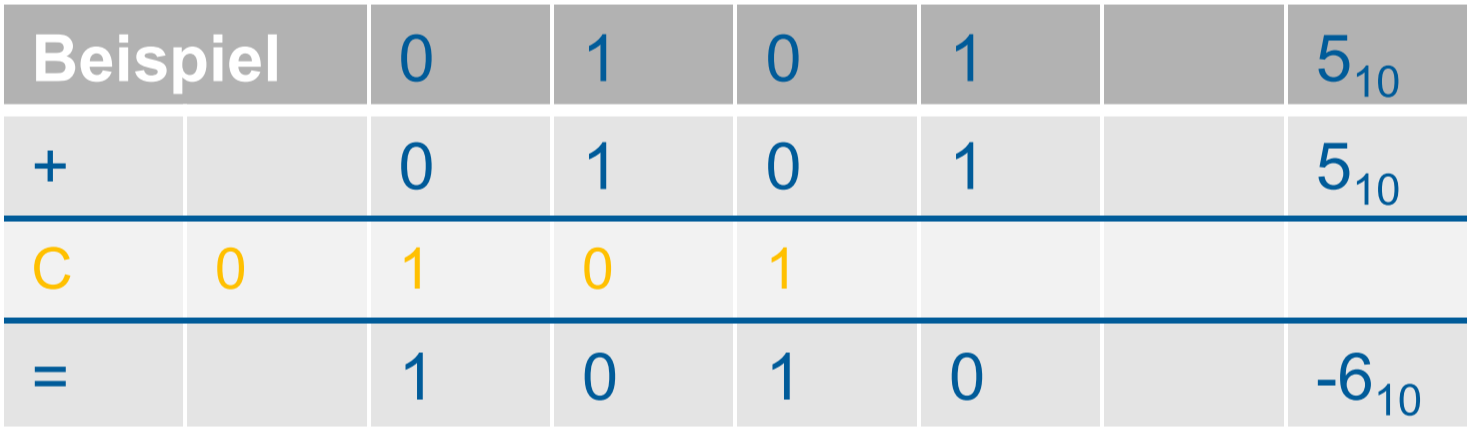
\includegraphics[width=0.45\textwidth]{pics/zahlensysteme/addition_posZahlen.png}
		%\columnbreak
		
		\subsubsection{Addition negativer Zahlen}
		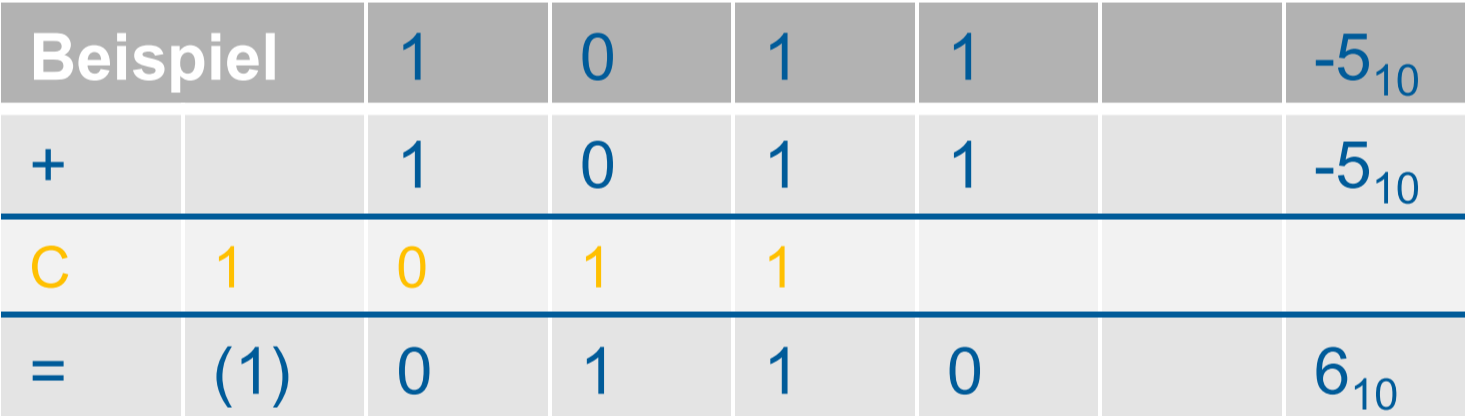
\includegraphics[width=0.45\textwidth]{pics/zahlensysteme/addition_negZahlen.png}
		%\columnbreak
	\end{multicols}